\documentclass{report}
\usepackage[dvipsnames]{xcolor}
\usepackage[american]{babel}
\usepackage{fontspec}
\usepackage[dvipsnames]{xcolor}
\usepackage{lmodern}
\usepackage{amssymb,amsmath}
\usepackage{comment} % enables the use of multi-line comments (\ifx \fi)
\usepackage{fullpage} % changes the margin
\usepackage{todonotes}
\usepackage{graphicx}
\usepackage{import}
\usepackage{multicol}
\usepackage{enumitem}


\usepackage[backend=biber,style=apa,url=false]{biblatex}
\addbibresource{SingingBirds.bib}
\DeclareLanguageMapping{american}{american-apa}

\usepackage{xifthen}
\usepackage{soul}
\sethlcolor{Apricot}
\newcommand\bla[1]{\ifthenelse{\isempty{#1}}{\hl{**~bla~bla~**}}{\hl{**~#1~**}}}
\usepackage[unicode=true]{hyperref}
\usepackage[all]{hypcap} % ref link to the top of the figure

\usepackage{csquotes} % Dependency for APA

\usepackage{titlesec}

\titleformat{\chapter}{\normalfont\huge}{\thechapter.}{20pt}{\Huge}


\hypersetup{breaklinks=true,
            pdfauthor={Paul Ecoffet},
            pdftitle={Master thesis Computational Model of birdsong learning},
            colorlinks=true,
            citecolor=blue,
            urlcolor=blue,
            linkcolor=black,
            pdfborder={0 0 0}
            }
\urlstyle{same} % don't use monospace font for urls


\title{Master Thesis - Computational model of Zebra Finch song learning and the
influence of sleep on it}
\author{Paul Ecoffet}
\date{The 6th of June, 2017}




\begin{document}
\maketitle

\begin{abstract}
The Zebra Finches are songbirds which learn the song of their tutor. They learn
it from 25 days post hatch (DPH) to 90 DPH \parencite{liu_juvenile_2004}. Zebra
finches are commonly used as a model of speech acquisition.

\textcite{deregnaucourt_how_2005} showed that sleep plays an important role in
the learning of tutor songs. Indeed, they showed that sleeping has a negative
impact on song restitution by zebra finches in the short term but a positive
impact on the long run. Song restitution is less complex and less similar to the
tutor song from one morning to the previous day evening, but the greater this
loss in performance was overall for one bird, the better this bird was able to
reproduce the tutor song at the end of its learning.

In addition to that, \textcite{dave_song_2000} have found neurons in the motor
cortex which fires sequences during sleep that correspond to their activity
pattern when the birds sing in adult zebra finches. This shows that motor
neurons that are highly correlated with bird's own song (BOS) are activated
during the night. These identified replays suggest that some learning may occur
during sleep that use past experiences.

Our hypothesis is that during its sleep, the zebra finch restructures the
knowledge it has acquired so far thanks to replay mechanisms. We hypothesize
that this restructuring can account for the loss of performance in the short
term and an improvement of performance in the long term.

The goal of this internship is to offer a model of the zebra finch song
learning which can explain different behavioral data observed such as the
correlation between the loss of performance every night and the overall
performance at the end of learning.
\end{abstract}

\tableofcontents

\chapter{Introduction}

\section{Zebra finch song learning}

The Zebra Finches are songbirds which learn the song of their tutor. They learn
it from 25 days post hatch (DPH) to 90 DPH \parencite{liu_juvenile_2004}.
Songbird and especially Zebra finches are commonly used as a comparison with
human about vocal development. Indeed, the song they produce are not innate
even though they have predispositions toward learning their songs. The songs
have rather complex structure, with a chaining of syllables that forms a
``motif'' \parencite{doupe_birdsong_1999, margoliash_evaluating_2002}.

These common characteristics can be studied easily with Zebra Finch. These birds
do learn their song quickly and they produce very stable and reproductible
songs. Zebra Finches learn only one song from a tutor and will sing it its whole
life. Therefore, the developmental trajectory of this learning can be tracked
and evaluation about the quality of the learning can be made.

The neuroanatomy of Zebra Finch has also been studied and the different
structures involved in singing has been identified. The neurological circuitries
of Zebra Finch studied.



Why model of speech acquisition:
* fast learning (90 days)
* Learning during development \cite{margoliash_offline_2003}
* Very reproductible result with a tutor song that the bird will mimic its whole
  life \cite{margoliash_sleep_2010}
    * Close ended learners vs open-ended learner \cite{margoliash_sleep_2010}
* Many-to-many relationship between auditory feedback and muscle outputs \cite{margoliash_offline_2003}

* Can be easily raised domesticaly \parencite{helekar_time_2013}
* More localised brain structure \parencite{helekar_time_2013}
    * Can study circuitries


The stages of learning
* subsong, plastic, cristallization \cite{margoliash_sleep_2010}


\section{Neurobiology}

Anatomy of the birdsong brain.

\section{Sleep}

\textcite{deregnaucourt_how_2005} showed that sleep plays an important role in
the learning of tutor songs. Indeed, they showed that sleeping has a negative
impact on song restitution by zebra finches in the short term but a positive
impact on the long run. Song restitution is less complex and less similar to the
tutor song from one morning to the previous day evening, but the greater this
loss in performance was overall for one bird, the better this bird was able to
reproduce the tutor song at the end of its learning.

\textcite{dave_song_2000} have found neurons in the motor cortex which fires
sequences during sleep that correspond to their activity pattern when the birds
sing in adult zebra finches. This shows that motor neurons that are highly
correlated with bird's own song (BOS) are activated during the night. These
identified replays suggest that some learning may occur during sleep that use
past experiences.

* Replays can explain learning \cite{margoliash_offline_2003}
* Consolidate learning
* Needed to reach new sounds \cite{margoliash_offline_2003}
* replays with weird burst inside \cite{margoliash_evaluating_2002}

\section{Sum up}
Our hypothesis is that during its sleep, the zebra finch restructures the
knowledge it has acquired so far thanks to replay mechanisms. We hypothesize
that this restructuring can account for the loss of performance in the short
term and an improvement of performance in the long term.

The goal of this internship is first of all to provide a model of the zebra
finch song learning with realistic constraints. This model will then allow us to
explore different strategies that the bird may use to learn the tutor song. The
strategies that we will test would have different prerequisites that could be
tested experimentally.

Thanks to this model, we are able to test easily different strategies of
learning during the day and during sleep. We are therefore able to look for
learning strategies that yield similar results as the observed data. If a
combination of strategies yield the correlation between the loss of performance
every night and the overall performance at the end of learning, we can
hypothesize that zebra finch are using similar learning strategies and we can
make new predictions that can be tested experimentally to test the robustness
of our model.

\section{Previous models for birdsong learning with Zebra Finches}

Even if the neurobiological structures involved in singing have been heavily
studied, only a few models of birdsong learning have already been proposed, even
less have been implemented.

Reinforcement learning is often evoked as the strategy the birds use to learn
their song \parencite{dave_song_2000,marler_three_1997}\todo{more ref}. Though,
the authors only talk very briefly about reinforcement learning and do not
really implement the birdsong learning algorithm with reinforcement learning.
They do not explain what would be the state space, the action space and the
reward function.

\textcite{marler_three_1997} built a computational model of Zebra Finch birdsong
learning. The computational model is based on a sound synthesizer, therefore
Coen's algorithm has to deal with real sounds. In his algorithm, the bird learns
the sensorimotor map of its vocal production. The bird does random motor
movement and group them according to the different characteristics the produced
sound has. With enough babbling, the simulated bird is able to reproduce its
tutor song. Interesting concepts are brought by Marler's approach. For instance,
he brought the concept of ``songemes'', the song equivalent of phonemes. A
syllables is composed of several songemes. Indeed, by having to build an
algorithm that actually produces songs, the notion of syllables or even notes is
not sufficient enough. Syllables and notes are revelant in the sensory space,
but not in the motor space. Songemes are described by Coen as the primitive
units of bird song. Though, Coen's model has several issues.\todo{list issues}

* Preference for same species songs \cite{margoliash_evaluating_2002,
marler_three_1997}
* \cite{marler_three_1997}
* \cite{coen_learning_2007} with a strange clustering technique



\chapter{Our proposed model}

\section{Synthesizer}

We want to build a model with realistic constraints, both in the computational
budget required by the bird to learn its song as of the actual material the
model deals with. We therefore uses a realistic zebra finch song synthesizer.
\textcite{perl_reconstruction_2011} built a realistic model of the Zebra Finch
vocal apparatus. They described with differential equations its behaviour,
taking into account parameters such as the length of the syrinx of the bird
\todo{more examples} and are able to reproduce accurately real zebra finches
song. The reproduction is good enough to activate bird's own song specific
neurons zebra finches have \parencite{boari_automatic_2015}.

The synthesizer takes as input a stream of two parameters: The air sac pressure,
that is how much air is flowing in the vocal apparatus of the bird, and
syringeal labial tension, which is equivalent to the vibration of our vocal
\todo{find the word}. These two values are changed by the muscles in the vocal
apparatus of the bird, and we can therefore infer that the motor command sent by
the bird brain to the muscles of its vocal apparatus have the purpose of
changing these values.

This synthesizer provides a very interesting framework to work with birdsong
learning. It constraints a realistic motor space and generates realistics songs
in the sensory space. Therefore, our algorithm works on real sounds and have to
find parameters that are roughly equivalent to the parameters send by the bird
to its muscles.


Our algorithm looks for the best values to parametrize the synthesizer.


\section{Global architecture}


\subsection{Terminology}

\begin{description}
  \item[Tutor song] The tutor song is the goal song the agent try to reproduce.
  \item[Song Model] A song model is the representation of the motor commands an
  agent has to produce a song. A song model is composed of several gestures,
  with the associated parameters and duration.
  \item[Song structure] The song structure is the agencement of the gestures.
  Without modifying the parameters of a gesture, the song structure can change
  by inserting a new gesture, deleting one or changing the length of a gesture.
  \item[Gesture] A gesture is the motor primitive of the song. A gesture
  is defined by its duration and motor command generator parameters.
  \item[Learning model] A learning model is an algorithm that modify Song Models
  so that they match better the tutor song. A learning model can be used either
  during ``days'' or ``nights''.
\end{description}

\subsection{Overview}

\subsection{Memorisation of the tutor song template}

We assumed the tutor song template was already known by the bird and that it has
a perfect access to it. This is consistent with results in the litterature.
Indeed, zebra finches need to listen to the tutor song only for a short critical
period which occurs a bit before the starting of their babbling, from 20DPH to
50 DPH \parencite{deregnaucourt_how_2005, margoliash_sleep_2010}. The encoding
of the tutor song is a separate event from the vocal imitation. We simplified
the tutor representation in our model by a full knowledge of the tutor song
characteristics, always accessible by the bird for comparison with its own
production.

\subsection{Song representations}

The agent has several song models that he works on. The song models is modified
throughout the learning so that the motor commands it describes generate
accurately the tutor song.

\subsubsection{Song architecture}

\begin{figure}
\center
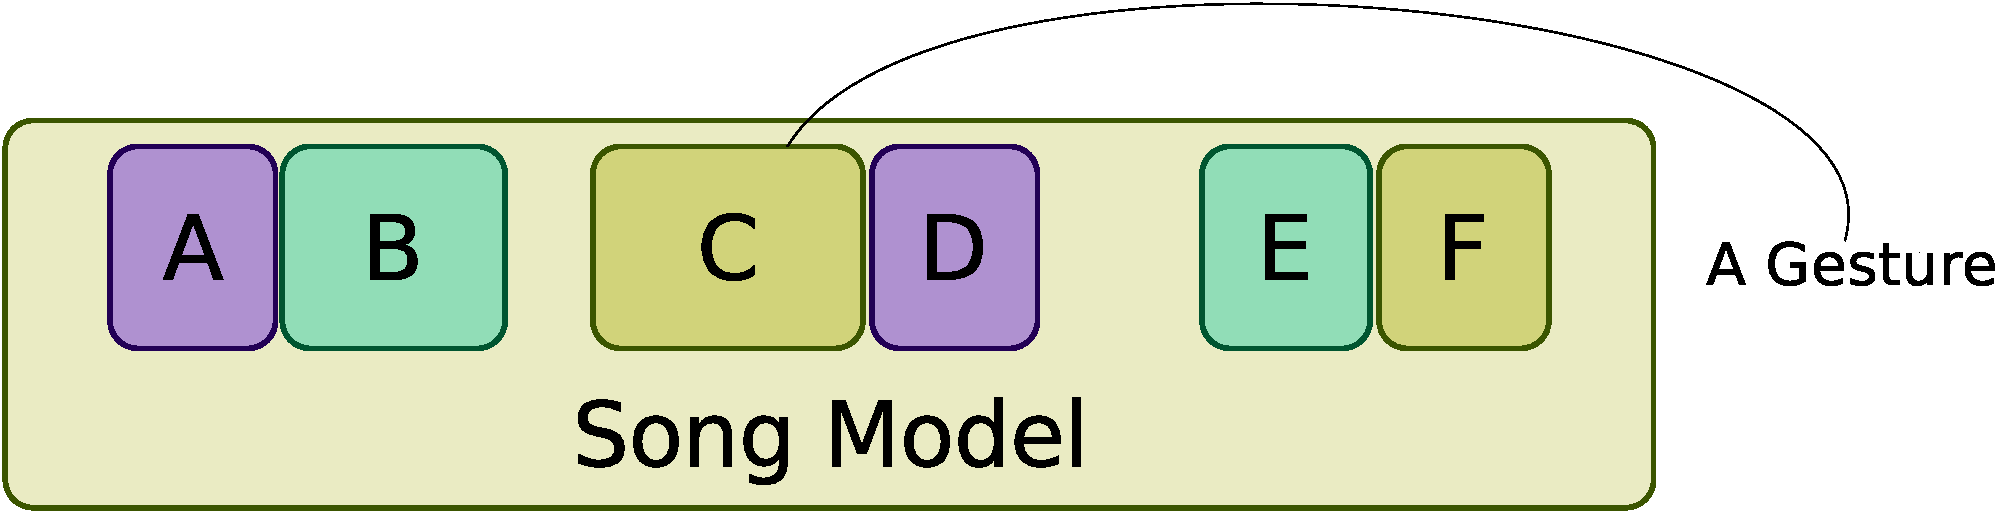
\includegraphics[width=0.8\linewidth]{song_model_architecture_schema}
\caption{Song Architecture\label{fig_song_arch}}
\end{figure}

The song architecture is determined by the number of gestures the song model
has, their durations and their starting point. Figure~\ref{fig_song_arch} shows
a simple song architecture.

\subsubsection{Gestures}

A gesture is determined by its length and the parameters that characterize the
generators for Syringeal Labial Tension (\(\alpha(t)\)) and Air sac Pressure
(\(\beta(t)\)).

\begin{align}
\alpha(t) &= a_\alpha \times t
  + b_\alpha + \sum_{i=1}^{3} c_{i,\alpha} \sin(\omega_{i,\alpha} \times 2\pi
  \times t + \phi_{i,\alpha}) + k_\alpha\\
\beta(t) &= a_\alpha \times t
  + b + c_\beta \sin(\omega_\beta \times 2\pi \times t + \phi_\beta) + k_\beta
\end{align}

\subsection{Day learning models}

* Default parameters found th

* hillclimbing
* Optimize gesture but not song structure


\subsection{Night learning models}

* Microbial GA
* Optimise only song structure, not gestures

\subsection{Parameters}

Fixed parameters
Optimized parameters

\subsection{Satellite Modules}

I built several side projects that were needed for the computational model to
work.



\subsubsection{Bird song analysis package}

The research community about birdsong uses a specific set of acoustic features
to describe songs. The community use the software Sound Analysis Pro (SAP) 2011
to extract them, or the Matlab equivalent Sound Analysis Toolbox (SAT)
\parencite{tchernichovski_procedure_2000}. SAP2011 is coded in C++ and only
compatible with Windows systems. It is also impossible to make calls to its
funcion with Python. In the same way, SAT was impossible to call from Python. I
have therefore ported the main functions of SAT and SAP to Python~3. I have
recoded all the feature extraction functions, the similarity measurement and
created plotting functions. I have also done plenty of optimisation to make the
code run as fast as possible, because most of the feature extractions are very
slow and I had issue with computation time on my project. The source code is
available at \url{https://github.com/PaulEcoffet/birdsonganalysis}. While I did
not get the exact same results as SAT, the results I have with this are
qualitatively equivalent. \todo{proof read}

\subsubsection{Synthesizer}

I used the synthesizer provided for download at \url{http://www.lsd.df.uba.ar}
\parencite{boari_automatic_2015}. The synthesizer was built in C and was not
very flexible. I have corrected a few ``bugs'' in the synthesizer (such as
injection of parameters at specific times) and make it integrable with Python
and Numpy thanks to Cython. The synthesizer was therefore callable by a Python
function. It generates sound waves with a stream of parameters $\alpha$ and
$\beta$. The source code for this synthesizer is available at
\url{https://github.com/PaulEcoffet/birdsynth}.

\section{Run methodology}

Grid search on cluster

How to create new models?



\chapter{Results}

\section{Syllables development trajectories}

\section{Influence of song model restructuration on learning}

\chapter{Discussion}

\chapter{Conclusion}

\printbibliography{}

\end{document}
